\chapter{맥스웰 방정식, 공변성, 그리고 전자기파}

\lectureoverview{전기장과 자기장은 로런츠 힘을 통해 하전 물질에 작용하지만, 물질도 전기장과 자기장을 만들어 재배열해야 합니다. 이번에는 전자기학의 이 상호적인 나머지 절반을 정식화하고, 맥스웰 방정식이 로런츠 공변임을 보이며, 파동 해를 유도한 다음, 국소 보존이 명확히 드러나는 형태로 전하와 전류를 다시 포함하겠습니다. 강의 전체에서 \(c=1\)인 단위를 사용합니다.}

\section{전자기학의 다른 절반}

먼저 이미 살펴본 부분부터 시작합시다. 전하 \(q\)인 입자가 전기장과 자기장 속에서 속도 \(\mathbf v\)로 움직이면, 힘은 다음과 같습니다.
\begin{equation}
\mathbf F=q\bigl(\mathbf E+\mathbf v\times\mathbf B\bigr).
\label{eq:lorentz-force-three}
\end{equation}
인자 \(q\)는 반드시 필요합니다. 전하가 없는 입자는 전자기력을 느끼지 않습니다. 입자가 순간적으로 정지해 있어도 전기장은 힘에 기여하지만, 자기장의 기여는 입자의 운동에 달려 있습니다.

방정식~\eqref{eq:lorentz-force-three}은 주어진 장이 물질에 어떤 작용을 하는지 알려 줍니다. 하지만 장을 결정하는 것이 무엇인지는 말해 주지 않습니다. 한 물체 주위의 전기장, 다른 물체 주위의 자기장, 또는 빈 공간을 따라 움직이는 파동은 무엇이 만들어 낼까요? 이 질문에 답하는 방정식이 맥스웰 방정식입니다.

\begin{figure}[H]
\centering
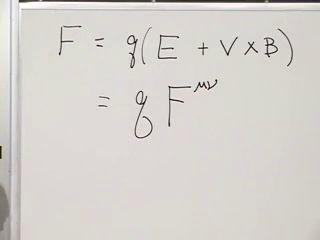
\includegraphics[width=0.62\textwidth]{lecture_58_figure_02.png}
\caption{3차원 로런츠 힘과 그 텐서 표현의 시작.}
\lectureframe{00:05:49}
\end{figure}

힘 법칙의 상대론적 형태에는 앞으로 필요한 표기법이 이미 담겨 있습니다.
\begin{equation}
f^\mu=qF^\mu{}_{\nu}u^\nu.
\label{eq:lorentz-force-four}
\end{equation}
여기서 \(u^\nu\)는 4-속도, \(f^\mu\)는 4-힘이며, \(F^{\mu\nu}\)는 \(\mathbf E\)와 \(\mathbf B\)로 구성한 반대칭 텐서입니다. 판서에는 우선 이 식의 개략적인 시작 부분만 나타나 있습니다. \(u^\nu\)와의 축약으로 빠져 있던 벡터가 더해져, 힘의 지표 하나가 자유 지표로 남습니다.

물질이 장에 다시 영향을 미쳐야 하는 데에는 물리적인 이유가 있습니다. 전자기파가 전하에 부딪히면 전하를 가속하고 에너지를 전달할 수 있습니다. 장은 전하에 영향을 주면서 전하는 장에 영향을 줄 수 없다면, 그 에너지가 어디서 빠져나오는지 설명할 길이 없습니다. 작용과 반작용만으로 논증이 끝나는 것은 아니지만, 에너지 보존을 생각하면 상호적인 결합은 불가피합니다.

\section{변화하는 원천은 교란을 내보낸다}

점전하는 그 위치에서 바깥쪽이나 안쪽을 향하는 전기장을 만듭니다. 도선의 전류--하전 입자들의 흐름--는 도선을 둘러싸고 회전하는 자기장을 만듭니다. 익숙한 이 정전기적·정자기적 그림만으로도 서로 다른 두 기하학적 형태를 볼 수 있습니다. 전기 플럭스는 전하에서 뻗어 나오고, 자기력선은 전류 주위를 감쌉니다.

이제 점전하를 갑자기 움직여 봅시다. 새 위치 근처에서는 전기장이 재배열되기 시작해야 하지만, 멀리 있는 관찰자는 그 움직임을 즉시 알 수 없습니다. 신호가 도달할 시간이 흐를 때까지 먼 곳에는 이전 장이 그대로 남습니다. 가까운 영역과 먼 영역 사이에는 장이 변하는 경계면이 이동합니다. 이렇게 이동하는 장의 재배열이 전자기 교란입니다.

전하를 왕복 운동시키면 재배열이 잇따라 일어나 전자기파를 이룹니다. 이것이 안테나의 기본 작동 원리입니다. 진동하는 전류가 장의 교란을 바깥으로 내보냅니다. 도선의 전류 방향을 뒤집어도 같은 논리로 자기장에 관한 그림을 얻습니다. \(\mathbf B\)의 회전 방향도 바뀌어야 하지만, 그 변화는 모든 곳에서 한꺼번에 나타나는 것이 아니라 전파됩니다.

이 인과적 그림은 맥스웰 방정식에 두 가지 조건을 요구합니다. 전하와 전류가 장의 원천이 되는 방식을 설명해야 하고, 장의 변화가 빛보다 빠르지 않게 전파될 수 있어야 합니다. 두 번째 조건은 상대성 이론을 검증하는 기준이기도 합니다. 맥스웰 방정식이 모든 관성계에서 같은 형태를 가지며 특정한 파동 속도를 함의한다면, 모든 관성계의 관찰자는 그 방정식에서 같은 속도를 얻어야 합니다.

\section{상대론적 파동 방정식 복습}

벡터장을 살펴보기 전에 스칼라장 \(\phi(\mathbf x,t)\)을 생각해 보자. 이는 시공간의 각 점에 하나의 수가 대응하는 장이다. 일계 미분 방정식
\begin{equation}
\partial_\mu\phi=0
\end{equation}
은 시공간의 모든 미분이 사라진다는 뜻이다. 그러면 장은 상수가 되어 파동을 전달할 수 없다. 비자명한 상대론적 파동 방정식에는 두 번의 미분이 들어간다.
\begin{equation}
\partial_\mu\partial^\mu\phi=0.
\end{equation}
여기서 사용한 부호 규약에 따르면
\begin{equation}
\left(\partial_t^2-\partial_x^2-\partial_y^2-\partial_z^2\right)\phi=0,
\label{eq:scalar-wave-four}
\end{equation}
또는 더 간결하게
\begin{equation}
\left(\partial_t^2-\nabla^2\right)\phi=0.
\end{equation}
이다. \(c=1\)로 두면 시간과 거리를 서로 양립하는 단위로 나타낼 수 있다. 일반적인 단위를 복원하면 시간에 대한 이계 미분항 옆에 \(1/c^2\)가 붙는다.

\(z\)축을 따라 진행하는 파동에서는 장이 \(z\)와 \(t\)에 의존하고, \(x\)나 \(y\)에는 의존하지 않습니다. 방정식~\eqref{eq:scalar-wave-four}은 다음과 같이 됩니다.
\begin{equation}
\left(\partial_t^2-\partial_z^2\right)\phi=0.
\label{eq:scalar-wave-one}
\end{equation}

\begin{figure}[H]
\centering
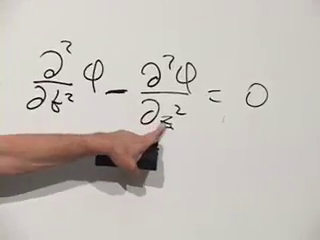
\includegraphics[width=0.56\textwidth]{lecture_58_figure_04.png}
\caption{전자기파의 모형으로 사용하는 1차원 스칼라 파동 방정식.}
\lectureframe{00:47:03}
\end{figure}

일반적인 진행파 해는 다음과 같습니다.
\begin{equation}
\phi(z,t)=f(z-t)+g(z+t).
\end{equation}
파형 \(f(z-t)\)은 위상이 일정한 점이 \(z-t=\text{constant}\)를 만족하므로 \(z\)가 증가하는 방향으로 이동합니다. 파형 \(g(z+t)\)은 반대 방향으로 이동합니다. 어느 파형도 정현파일 필요는 없습니다. 충분히 매끄러운 형태라면 모양을 바꾸지 않고 그대로 이동합니다.

그렇지만 정현파를 사용하면 편리합니다.
\begin{equation}
\phi(z,t)=A\cos\!\bigl(k(z-t)\bigr).
\end{equation}
파수 \(k\)는 파장을 결정합니다.
\begin{equation}
\lambda=\frac{2\pi}{k}.
\end{equation}
\(k\)가 크면 공간적으로 빠르게 진동하고 파장이 짧아집니다. \(k\)가 작으면 파장이 길어집니다. 곧 이 파형들은 \(\mathbf E\)와 \(\mathbf B\)의 성분이 됩니다.

\section{맥스웰 방정식에 필요한 벡터 미적분}

맥스웰 방정식에는 내적, 외적, 발산, 회전이 등장합니다. 뒤에서 성분별 계산에 바로 이 형태들을 사용하므로, 표기법을 한 번 다시 정리해 두겠습니다.

일반적인 3차원 벡터 \(\mathbf a\)와 \(\mathbf b\)에 대해 내적은 스칼라입니다.
\begin{equation}
\mathbf a\cdot\mathbf b
=a_xb_x+a_yb_y+a_zb_z.
\end{equation}
외적은 또 다른 벡터입니다.
\begin{align}
(\mathbf a\times\mathbf b)_x&=a_yb_z-a_zb_y,\\
(\mathbf a\times\mathbf b)_y&=a_zb_x-a_xb_z,\\
(\mathbf a\times\mathbf b)_z&=a_xb_y-a_yb_x.
\end{align}
나머지 성분은 순환 순서 \(x\to y\to z\to x\)에 따라 얻습니다.

미분 연산자
\begin{equation}
\boldsymbol\nabla=
\left(\partial_x,\partial_y,\partial_z\right).
\end{equation}
를 도입합시다. 각 성분은 보통 수가 아니라 연산자이지만, 내적과 외적의 형태를 그대로 사용할 수 있습니다. 벡터장 \(\mathbf A\)에 대해,
\begin{equation}
\boldsymbol\nabla\cdot\mathbf A
=\partial_xA_x+\partial_yA_y+\partial_zA_z
\label{eq:divergence}
\end{equation}
은 발산이고,
\begin{align}
(\boldsymbol\nabla\times\mathbf A)_x
 &=\partial_yA_z-\partial_zA_y,\\
(\boldsymbol\nabla\times\mathbf A)_y
 &=\partial_zA_x-\partial_xA_z,\\
(\boldsymbol\nabla\times\mathbf A)_z
 &=\partial_xA_y-\partial_yA_x
\label{eq:curl}
\end{align}
은 회전의 성분입니다.

기하학적 의미는 수식만큼이나 중요합니다. 벡터장이 원천으로부터 바깥쪽으로 흘러나오는 듯한 곳에서는 발산이 양수입니다. 벡터장이 회전하는 곳에는 회전이 있습니다. 점전하의 방사형 전기장은 발산을, 전류가 흐르는 도선을 감싸는 자기장은 회전을 보여 줍니다. 공간적으로 일정한 벡터장에는 둘 다 없습니다.

\section{진공에서의 맥스웰 방정식}

전하와 전류가 없을 때 맥스웰 방정식은 다음과 같습니다.
\begin{align}
\boldsymbol\nabla\times\mathbf E&=-\partial_t\mathbf B,
\label{eq:faraday-vac}\\
\boldsymbol\nabla\cdot\mathbf B&=0,
\label{eq:gauss-b-vac}\\
\boldsymbol\nabla\times\mathbf B&=\partial_t\mathbf E,
\label{eq:ampere-vac}\\
\boldsymbol\nabla\cdot\mathbf E&=0.
\label{eq:gauss-e-vac}
\end{align}
두 회전 방정식은 \(\mathbf E\)와 \(\mathbf B\)를 거의 맞바꾼 형태지만, 중요한 마이너스 부호 하나가 둘을 구별합니다. 두 발산 방정식은 고려하는 진공 영역에 어느 장에도 원천이 없음을 말합니다. 전기 원천을 다시 포함해도 자기장의 발산은 여전히 0입니다. 일반적인 전자기학에는 자기 전하가 없습니다.

\begin{figure}[H]
\centering
\includegraphics[width=0.76\textwidth]{lecture_58_figure_06.png}
\caption{전기장과 자기장 사이의 거의 대칭적인 관계가 드러나도록 배열한 진공 맥스웰 방정식 네 개.}
\lectureframe{00:27:30}
\end{figure}

전하 밀도 \(\rho\)는 결국 방정식~\eqref{eq:gauss-e-vac}의 우변에 있는 0을 대신하고, 전류 밀도 \(\mathbf J\)는 방정식~\eqref{eq:ampere-vac}에 들어갑니다. 잠시 이 항들을 미뤄 두겠습니다. 원천이 없는 방정식은 복잡한 항을 최소화한 채 변환 구조와 파동이 생기는 원리를 드러냅니다.

이 방정식들은 아인슈타인의 문제도 한층 선명하게 보여 줍니다. 파동을 따라 움직이는 갈릴레이 관찰자라면 속도를 빼서 파동 속도가 더 작게 측정될 것이라고 예상할 것입니다. 하지만 같은 맥스웰 방정식이 모든 관성계에서 성립한다면, 각 관찰자는 그 방정식에서 동일한 단위 파동 속도를 얻습니다. 해결책은 관성계마다 파동 방정식을 바꾸는 것이 아닙니다. 로런츠 변환을 사용하고, 변환 법칙이 이미 알려진 대상들로 맥스웰 방정식을 나타내는 것입니다.

\section{하나의 텐서로 묶이는 전기장과 자기장}

전기장과 자기장을 반대칭 장 텐서로 결합하면 다음과 같다.
\begin{equation}
F^{\mu\nu}=
\begin{pmatrix}
0   & -E_x & -E_y & -E_z\\
E_x & 0    & -B_z & B_y\\
E_y & B_z  & 0    & -B_x\\
E_z & -B_y & B_x  & 0
\end{pmatrix},
\label{eq:l0203-field-tensor}
\end{equation}
행과 열의 순서는 \(t,x,y,z\)이다. 반대칭성
\begin{equation}
F^{\mu\nu}=-F^{\nu\mu},
\end{equation}
에 의해 대각 성분은 영이 되고, 행렬의 아래쪽 절반은 위쪽 절반으로 결정된다. 시간과 공간에 해당하는 성분에는 \(\mathbf E\)가 들어가며, 공간에만 해당하는 성분에는 \(\mathbf B\)가 들어간다.

\begin{figure}[H]
\centering
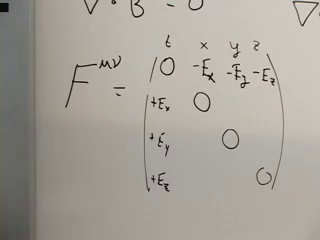
\includegraphics[width=0.58\textwidth]{lecture_58_figure_03.png}
\caption{전기장과 자기장 성분을 모두 포함한 완성된 전자기장 텐서.}
\lectureframe{00:32:05}
\end{figure}

\(F^{\mu\nu}\)가 중요한 이유는 장 성분 여섯 개를 하나의 행렬에 넣을 수 있다는 데 그치지 않습니다. 로런츠 변환 아래에서 이 텐서는 2계 텐서로 변환됩니다. 따라서 관찰자마다 측정하는 전기장과 자기장은 전체 텐서가 일관되게 변환되는 데 필요한 방식으로 서로 섞입니다.

또 다른 반대칭 텐서인 쌍대 장 텐서 \(\widetilde F^{\mu\nu}\)도 있습니다. 현재의 규약에서는 방정식~\eqref{eq:l0203-field-tensor}에 다음 치환을 적용해 얻습니다.
\begin{equation}
\mathbf E\longmapsto-\mathbf B,
\qquad
\mathbf B\longmapsto\mathbf E.
\label{eq:dual-replacement}
\end{equation}
따라서
\begin{equation}
\widetilde F^{\mu\nu}=
\begin{pmatrix}
0    & B_x  & B_y  & B_z\\
-B_x & 0    & -E_z & E_y\\
-B_y & E_z  & 0    & -E_x\\
-B_z & -E_y & E_x  & 0
\end{pmatrix}.
\label{eq:dual-tensor}
\end{equation}
방정식~\eqref{eq:dual-replacement}의 부호는 중요합니다. 강의에서는 먼저 말로 두 장을 맞바꾸어 보다가 부호가 맞지 않음을 알아차리고, 행렬을 완성하기 전에 이를 바로잡습니다.

\begin{figure}[H]
\centering
\includegraphics[width=0.58\textwidth]{lecture_58_figure_07.png}
\caption{필요한 부호를 포함해 전기장과 자기장 성분을 교환하며 구성하는 쌍대 텐서.}
\lectureframe{00:35:45}
\end{figure}

\section{공변적인 진공 방정식}

맥스웰 방정식은 각각 미분 하나를 포함합니다. 2계 텐서에서 한 미분 지표를 축약하면 자유 지표 하나가 남으므로, 공변적인 형태로 자연스럽게 생각할 수 있는 식은 다음과 같습니다.
\begin{align}
\partial_\mu F^{\mu\nu}&=0,
\label{eq:maxwell-covariant-vac}\\
\partial_\mu\widetilde F^{\mu\nu}&=0.
\label{eq:maxwell-dual-vac}
\end{align}
\(\nu\)를 하나의 고정된 값으로 두면 방정식~\eqref{eq:maxwell-covariant-vac}은 하나의 방정식입니다. \(\nu\)는 \(t,x,y,z\) 가운데 하나일 수 있으므로, 이 식은 스칼라 방정식 네 개를 묶습니다. 방정식~\eqref{eq:maxwell-dual-vac}은 나머지 네 개를 묶습니다. 이는 앞서 나열한 벡터 회전 방정식 두 개와 스칼라 발산 방정식 두 개에 해당합니다.

간결한 표기는 익숙한 방정식을 재현할 때만 유용하다. \(\nu=z\)으로 두면
\begin{align}
\partial_\mu F^{\mu z}
&=\partial_tF^{tz}
  +\partial_xF^{xz}
  +\partial_yF^{yz}
  +\partial_zF^{zz}\\
&=-\partial_tE_z+\partial_xB_y-\partial_yB_x\\
&=-\partial_tE_z+
  \bigl(\boldsymbol\nabla\times\mathbf B\bigr)_z.
\end{align}
항 \(F^{zz}\)는 반대칭성 때문에 영이 된다. 결과를 영으로 놓으면 \(z\) 성분에 해당하는 다음 식을 얻는다.
\begin{equation}
\boldsymbol\nabla\times\mathbf B=\partial_t\mathbf E.
\end{equation}
지표를 순환시키면 \(x\) 및 \(y\) 성분도 얻어진다.

\begin{figure}[H]
\centering
\includegraphics[width=0.76\textwidth]{lecture_58_figure_08.png}
\caption{공변 장 방정식을 성분별로 전개하면, 대각 텐서 성분은 사라지고 나머지 항들이 맥스웰 방정식을 재구성한다.}
\lectureframe{00:43:30}
\end{figure}

이제 시간 성분을 살펴봅시다.
\begin{align}
\partial_\mu F^{\mu t}
&=\partial_tF^{tt}
  +\partial_xF^{xt}
  +\partial_yF^{yt}
  +\partial_zF^{zt}\\
&=\partial_xE_x+\partial_yE_y+\partial_zE_z\\
&=\boldsymbol\nabla\cdot\mathbf E.
\end{align}
따라서 방정식~\eqref{eq:gauss-e-vac}을 줍니다. 쌍대 텐서에 대해서도 같은 검산을 하면
\(\boldsymbol\nabla\cdot\mathbf B=0\)와
\(\boldsymbol\nabla\times\mathbf E=-\partial_t\mathbf B\)를 얻습니다.

이제 간결한 방정식들은 단순히 추측한 것이 아니라 실제로 도출되었습니다. 자유 지표의 구조를 보면 이 식들이 4-벡터 방정식임을 알 수 있습니다. 따라서 로런츠 변환은 성분을 바꾸지만 형태는 바꾸지 않습니다. 이것이 진공 맥스웰 방정식이 모든 관성계에서 동일한 형태를 갖는다는 말의 정확한 의미입니다.

\section{1계 방정식에서 파동으로}

맥스웰 방정식에는 1계 미분만 들어가지만 파동 방정식에는 2계 미분이 들어갑니다. 이 겉보기의 불일치는 맥스웰 이론이 두 장을 결합한다는 점에서 해소됩니다. \(\mathbf E\)와 \(\mathbf B\)에 대한 1계 방정식 두 개를 결합하면 둘 중 어느 한 장만으로 나타낸 2계 방정식을 얻을 수 있습니다.

방정식~\eqref{eq:ampere-vac}을 시간에 대해 미분합시다.
\begin{equation}
\partial_t^2\mathbf E
=\boldsymbol\nabla\times\partial_t\mathbf B.
\end{equation}
패러데이 법칙은 \(\mathbf B\)의 시간 미분을 줍니다.
\begin{equation}
\partial_t\mathbf B=-\boldsymbol\nabla\times\mathbf E,
\end{equation}
따라서
\begin{equation}
\partial_t^2\mathbf E
=-\boldsymbol\nabla\times
  \bigl(\boldsymbol\nabla\times\mathbf E\bigr).
\label{eq:double-curl}
\end{equation}

판서에서는 외워 둔 항등식을 바로 쓰는 대신 성분 하나를 직접 계산합니다. \(x\) 성분은 다음과 같습니다.
\begin{align}
\bigl[\boldsymbol\nabla\times
(\boldsymbol\nabla\times\mathbf E)\bigr]_x
&=\partial_y(\boldsymbol\nabla\times\mathbf E)_z
 -\partial_z(\boldsymbol\nabla\times\mathbf E)_y\\
&=\partial_y(\partial_xE_y-\partial_yE_x)\\
&\quad-\partial_z(\partial_zE_x-\partial_xE_z)\\
&=\partial_x(\partial_yE_y+\partial_zE_z)
 -\partial_y^2E_x\\
&\quad-\partial_z^2E_x.
\end{align}
\(\partial_x^2E_x\)를 더하고 빼서 발산을 드러냅시다.
\begin{align}
\bigl[\boldsymbol\nabla\times
(\boldsymbol\nabla\times\mathbf E)\bigr]_x
&=\partial_x(\boldsymbol\nabla\cdot\mathbf E)
 -\nabla^2E_x.
\label{eq:double-curl-x}
\end{align}
진공에서는 \(\boldsymbol\nabla\cdot\mathbf E=0\)입니다. 방정식~\eqref{eq:double-curl}와 \eqref{eq:double-curl-x}를 결합하면
\begin{equation}
\left(\partial_t^2-\nabla^2\right)E_x=0.
\label{eq:ex-wave}
\end{equation}을 얻습니다.

\begin{figure}[H]
\centering
\includegraphics[width=0.72\textwidth]{lecture_58_figure_09.png}
\caption{성분 계산을 통해 \(E_x\)에 대한 파동 방정식을 얻는다.}
\lectureframe{00:57:10}
\end{figure}

같은 계산을 \(E_y\)와 \(E_z\)에도 적용할 수 있으며, 유사하게 항을 소거하면 다음 식을 얻습니다.
\begin{equation}
\left(\partial_t^2-\nabla^2\right)\mathbf B=0.
\end{equation}
따라서 전기장과 자기장은 빈 공간을 파동으로 전파할 수 있습니다. 사용하는 단위계에서는 그 속도가 1이며, 통상적인 단위를 복원하면 속도는 \(c\)입니다.

\section{평면파와 편광}

양의 \(z\) 방향으로 진행하는 간단한 파동을 구성해 봅시다.
\begin{equation}
\mathbf E(z,t)
=\widehat{\mathbf x}\,E_0
  \cos\!\bigl(k(z-t)\bigr).
\label{eq:plane-e}
\end{equation}
파형은 모양을 바꾸지 않고 \(z\) 방향으로 이동합니다. 전기장이 \(x\)축을 따라 있으므로 이 파동의 선형 편광 방향은 \(x\)입니다. 예를 단순하게 유지하려고 \(E_y=0\)로 두었습니다. 두 번째 횡편광을 추가할 수도 있습니다.

종방향 성분은 같은 방식으로 자유롭지 않습니다. 파동이 \(z\)와 \(t\)에만 의존하므로,
\begin{equation}
\boldsymbol\nabla\cdot\mathbf E
=\partial_zE_z=0.
\end{equation}
따라서 \(E_z\)는 상수일 수 있지만, 변하는 파형을 포함할 수는 없습니다. 균일한 배경장은 따로 더하거나 제거할 수 있으며, 전파하는 복사에는 속하지 않습니다. 파동 자체는 횡방향입니다.
\begin{equation}
\mathbf E_{\mathrm{wave}}\cdot\widehat{\mathbf z}=0.
\end{equation}

패러데이 법칙으로 자기장이 정해진다. 식~\eqref{eq:plane-e}에서 \(\boldsymbol\nabla\times\mathbf E\)의 영이 아닌 성분은 \(y\) 성분뿐이며,
\begin{equation}
(\boldsymbol\nabla\times\mathbf E)_y=\partial_zE_x.
\end{equation}
따라서 \(\partial_t\mathbf B\)는 \(y\) 방향을 향하고, 이에 부합하는 선택은 다음과 같다.
\begin{equation}
\mathbf B(z,t)
=\widehat{\mathbf y}\,E_0
  \cos\!\bigl(k(z-t)\bigr).
\label{eq:plane-b}
\end{equation}
이 단위계에서는 전기장과 자기장의 진폭이 같다. 두 장의 방향 관계는 다음과 같다.
\begin{equation}
\mathbf E\perp\mathbf B,
\qquad
\mathbf E\perp\widehat{\mathbf z},
\qquad
\mathbf B\perp\widehat{\mathbf z},
\qquad
\mathbf E\times\mathbf B\parallel\widehat{\mathbf z}.
\end{equation}

\begin{figure}[H]
\centering
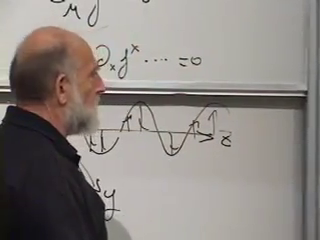
\includegraphics[width=0.70\textwidth]{lecture_58_figure_05.png}
\caption{완성된 횡전자기파 판서 그림. 전기장과 자기장의 진동 방향은 서로 수직이며 전파 방향에도 수직이다.}
\lectureframe{01:05:25}
\end{figure}

\begin{figure}[H]
\centering
\scalebox{0.90}{%
\begin{tikzpicture}[x=1cm,y=1cm,>=Latex]
  \draw[->,thick] (0,0) -- (8.2,0) node[right] {$z$};
  \draw[->,thick] (0,-1.6) -- (0,1.7) node[above] {$x$};
  \draw[->,thick] (0,0) -- (-1.15,-0.8) node[below left] {$y$};
  \draw[blue!70!black,thick,domain=0:7.5,samples=120]
    plot (\x,{0.95*sin(90*\x)});
  \foreach \z/\s in {0.8/1,2.8/-1,4.8/1,6.8/-1}{
    \draw[->,green!45!black,thick]
      (\z,0) -- ++({-0.55*\s},{-0.38*\s});
  }
  \node[blue!70!black] at (6.9,1.25) {$\mathbf E$};
  \node[green!45!black] at (5.2,-1.05) {$\mathbf B$};
  \draw[->,very thick] (6.2,1.55) -- (7.7,1.55)
    node[midway,above] {propagation};
\end{tikzpicture}
}
\caption{\(\mathbf E\)와 \(\mathbf B\)는 서로 수직이고,
전파 방향에도 수직입니다.}
\end{figure}

이것이 빛과 진공 속 모든 전자기 복사의 특성입니다. 파동을 만들어 낸 방정식이 로런츠 공변이므로, 다른 관성계의 관찰자도 횡방향 전기장과 자기장을 가진 전자기파가 \(c\)의 속도로 움직인다고 기술합니다.

\section{전하 밀도와 전류 밀도}

이제 잠시 미뤄 두었던 원천을 다시 포함하겠습니다. 한 영역에 하전 입자가 많이 있을 때는 이들을 연속적인 전하 밀도로 거시적으로 묘사하는 것이 편리합니다.
\begin{equation}
\rho(\mathbf x,t)=\frac{dQ}{dV}.
\end{equation}
분자로 이루어진 물을 연속적인 유체로 취급하는 것과 비슷한 근사입니다. 양전하와 음전하는 서로 반대 부호로 기여하므로, \(\rho\)는 단위 부피당 알짜 전하입니다.

정해진 영역 \(V\) 안의 전하는 다음과 같습니다.
\begin{equation}
Q_V(t)=\int_V\rho(\mathbf x,t)\,dV.
\label{eq:charge-volume}
\end{equation}
밀도는 위치와 시간에 따라 변할 수 있습니다. 한곳에 모여 있던 전하가 빠져나가면 그곳의 국소 밀도는 변합니다. 그러나 밀도가 임의의 방식으로 변할 수는 없습니다. 자연에서는 전하가 보존됩니다.

전역적인 보존만으로는 조건이 너무 약합니다. 전체 전하가 그대로인 채 지구에서 전하가 사라졌다가 같은 순간 화성에서 다시 나타나는 것도 허용하게 되기 때문입니다. 더 강한 조건은 국소적입니다. 전하는 그 사이 공간을 흐르지 않고서는 한곳을 떠나 다른 곳에 도달할 수 없습니다.

그 흐름을 기술하기 위해 방향을 정한 미소 면적 요소
\begin{equation}
d\boldsymbol\sigma=\widehat{\mathbf n}\,d\sigma.
\end{equation}
를 생각합시다. 크기는 면적이고 방향은 면에 수직입니다. 전류 밀도 \(\mathbf J\)는 이 요소를 단위 시간에 통과하는 전하가 다음과 같도록 정의합니다.
\begin{equation}
\frac{dQ}{dt}=\mathbf J\cdot d\boldsymbol\sigma.
\label{eq:current-flux-element}
\end{equation}
\(\mathbf J\)의 크기는 단위 면적·단위 시간당 전하량이며, 방향은 양전하가 흐르는 방향입니다.

\begin{figure}[H]
\centering
\includegraphics[width=0.64\textwidth]{lecture_58_figure_10.png}
\caption{방향이 정해진 면적 요소와 플럭스 인자 \(d\boldsymbol\sigma\cdot\mathbf J\).}
\lectureframe{01:18:15}
\end{figure}

내적은 면에 수직인 성분만 골라냅니다. 면에 접하는 전류는 어느 쪽으로도 면을 통과하지 않으므로 기여가 0입니다. 면의 법선과 나란한 전류는 크기가 일정할 때 플럭스가 최대입니다. 도선의 전류는 한 가지 특수한 경우일 뿐이며, \(\mathbf J\)는 판을 통과하거나 3차원 공간 전체를 흐르는 전하도 기술할 수 있습니다.

\section{국소 보존과 연속 방정식}

공간에서 영역 \(V\)를 고정하고, 그 닫힌 경계 \(\partial V\)의 모든 요소가 바깥쪽을 향하도록 방향을 정합시다. 순유출 전류가 있으면 내부 전하는 감소합니다.
\begin{equation}
\frac{dQ_V}{dt}
=-\oint_{\partial V}\mathbf J\cdot d\boldsymbol\sigma.
\label{eq:integral-conservation}
\end{equation}
마이너스 부호는 단순한 규약이 아니라 물리적 의미를 가집니다. 바깥쪽으로 나가는 양의 플럭스는 영역 안의 양전하를 줄입니다. 방정식~\eqref{eq:charge-volume}을 사용하면,
\begin{equation}
\int_V\partial_t\rho\,dV
=-\oint_{\partial V}\mathbf J\cdot d\boldsymbol\sigma.
\label{eq:integral-continuity-one}
\end{equation}

\begin{figure}[H]
\centering
\includegraphics[width=0.72\textwidth]{lecture_58_figure_11.png}
\caption{면 플럭스를 부피에 관한 식으로 바꾼 뒤 얻은 고정 영역의 보존 법칙.}
\lectureframe{01:29:00}
\end{figure}

발산 정리라고도 부르는 가우스 정리는 닫힌 면을 통과하는 플럭스를 내부의 발산과 연결합니다.
\begin{equation}
\oint_{\partial V}\mathbf A\cdot d\boldsymbol\sigma
=\int_V\boldsymbol\nabla\cdot\mathbf A\,dV.
\label{eq:divergence-theorem}
\end{equation}
그릇 안의 여러 지점에서 물을 주입하는 숨은 관을 떠올려 볼 수 있습니다. 발산은 관 끝에서 물이 나오는 국소적인 비율을 나타내고, 면적분은 그릇 밖으로 나가는 물의 총량을 나타냅니다. 내부에서 바깥쪽 흐름으로 생성된 물은 결국 경계를 통과해야 합니다.

식~\eqref{eq:divergence-theorem}을 \(\mathbf J\)에 적용하면
\begin{equation}
\int_V
\left(\partial_t\rho+\boldsymbol\nabla\cdot\mathbf J\right)dV=0.
\end{equation}
이 관계는 가능한 모든 영역 \(V\)에 대해 성립한다. 따라서 피적분함수는 각 점에서 영이어야 한다.
\begin{equation}
\boxed{\partial_t\rho+\boldsymbol\nabla\cdot\mathbf J=0.}
\label{eq:continuity-three}
\end{equation}

\begin{figure}[H]
\centering
\includegraphics[width=0.72\textwidth]{lecture_58_figure_12.png}
\caption{성분별로 쓴 국소 연속 방정식.}
\lectureframe{01:29:50}
\end{figure}

방정식~\eqref{eq:continuity-three}은 국소 보존이 요구하는 내용을 정확히 말해 줍니다. 한 점 또는 작은 영역에서 전하 밀도가 감소한다면 전류가 그곳에서 바깥으로 발산해야 합니다. 전류가 안쪽으로 모이면 전하 밀도는 증가합니다.

밀도와 전류는 자연스럽게 4-전류를 이룹니다.
\begin{equation}
J^\mu=(\rho,J_x,J_y,J_z)
\label{eq:four-current}
\end{equation}
\(c=1\) 단위계에서 연속 방정식은 로런츠 스칼라 방정식이 됩니다.
\begin{equation}
\partial_\mu J^\mu=0.
\label{eq:continuity-four}
\end{equation}
상대론적 분포의 흐름은 한 입자의 4-속도와 마찬가지로 4-벡터처럼 변환해야 합니다. 방정식~\eqref{eq:continuity-four}은 모든 관성계에서 국소 전하 보존이 성립하게 합니다.

\section{원천이 있는 맥스웰 방정식}

전하와 전류를 다시 포함하면 다음과 같습니다.
\begin{align}
\boldsymbol\nabla\cdot\mathbf E&=\rho,
\label{eq:gauss-e-source}\\
\boldsymbol\nabla\cdot\mathbf B&=0,\\
\boldsymbol\nabla\times\mathbf E&=-\partial_t\mathbf B,\\
\boldsymbol\nabla\times\mathbf B&=\partial_t\mathbf E+\mathbf J.
\label{eq:ampere-source}
\end{align}
전기 원천이 들어가는 방정식들은 다음 식으로 간결해집니다.
\begin{equation}
\boxed{\partial_\mu F^{\mu\nu}=J^\nu,}
\label{eq:maxwell-source-covariant}
\end{equation}
자기장에 대한 원천 없는 두 방정식은 그대로입니다.
\begin{equation}
\boxed{\partial_\mu\widetilde F^{\mu\nu}=0.}
\label{eq:maxwell-dual-source}
\end{equation}

\begin{figure}[H]
\centering
\includegraphics[width=0.78\textwidth]{lecture_58_figure_13.png}
\caption{원천이 있는 맥스웰 방정식과 그 공변 형태 \(\partial_\mu F^{\mu\nu}=J^\nu\).}
\lectureframe{01:34:00}
\end{figure}

방정식~\eqref{eq:maxwell-source-covariant}의 시간 성분은 다음과 같습니다.
\begin{equation}
\partial_\mu F^{\mu t}=J^t=\rho,
\end{equation}
앞서 수행한 성분 계산에 따르면 좌변은 \(\boldsymbol\nabla\cdot\mathbf E\)가 됩니다. 세 공간 성분은 다음을 재현합니다.
\(\boldsymbol\nabla\times\mathbf B=\partial_t\mathbf E+\mathbf J\)

유용한 일관성 검산도 가능합니다. \(\partial_\nu\)를 방정식~\eqref{eq:maxwell-source-covariant}에 적용하면 다음을 얻습니다.
\begin{equation}
\partial_\nu J^\nu
=\partial_\nu\partial_\mu F^{\mu\nu}=0,
\end{equation}
두 미분은 \(\mu\leftrightarrow\nu\)에 대해 대칭인 반면 \(F^{\mu\nu}\)는 반대칭이기 때문입니다.\editorialnote{이 짧은 일관성 검산은 공변 방정식에서 바로 따라 나오며, 원천이 있는 맥스웰 방정식이 연속 방정식을 자동으로 만족하는 이유를 명시적으로 보여 줍니다.}

이제 상호적인 구조가 완성되었습니다. 텐서 힘 법칙
\(f^\mu=qF^\mu{}_\nu u^\nu\)은 장이 전하에 어떻게 작용하는지 기술하고, 방정식~\eqref{eq:maxwell-source-covariant}은 전하와 전류가 장을 어떻게 만들어 내는지 기술합니다. 둘 다 텐서 방정식입니다. 진공에서는 같은 장 방정식이 \(c\)의 속도로 움직이는 횡파를 낳습니다. 이처럼 로런츠 공변성과 전자기파 방정식은 이 구성을 이끈 출발점에서 만납니다. 모든 관성계의 관찰자는 같은 전자기 법칙과 같은 빛의 속도를 얻습니다.
